\section*{Komplekse tal}
%%
%%
\begin{opgave}[1]{Den komplekse plan}
Tegn følgende komplekse tal i den komplekse plan.
\opg $z = 5$.
\opg $z = -3i$.
\opg $z = 4 + 7i$.
\opg $z = -3 - 2i$.
\end{opgave}
%%
%%
\begin{opgave}[1]{Regning med komplekse tal}
I denne opgave kigger vi på de komplekse tal:
\begin{align*}
z_1 &= 3 + 2i \, , \\
z_2 &= -6+i \, , \\ 
z_3 &= 1 - 5i \, , \\
z_4 &= -4 + 3i \, .
\end{align*}
\opg Beregn $z_1+z_2$ og $z_3+z_4$.
\opg Beregn $z_1-z_2$ og $z_3-z_4$.
\opg Beregn $z_1z_2$ og $z_3z_4$.
\opg Beregn $z_1/z_2$ og $z_3/z_4$.
\opg Beregn $\abs{z_1}$ og $\abs{z_2}$ samt $\abs{z_3 z_4}^2$. 
\end{opgave}
%%
%%
\begin{opgave}[2]{Regneregler for modulus og normkvadratet}
I denne opgave skal vi kigge på de regneregler for modulus samt normkvadratet for komplekse tal, der er  præsenteret i matematikafsnittet.
\opg Eftervis formlerne for modulus \eqref{k-modulus_regneregler1}, \eqref{k-modulus_regneregler2} og \eqref{k-modulus_regneregler3}.
\opg Eftervis formlen for normkvadratet \eqref{k-normkvadrat}.\\ \\  
\end{opgave}
%%
%%
\begin{opgave}[2]{Komplekse ligninger}
Løs de følgende komplekse ligninger.
\opg $\dfrac{z-2}{z+1} = 3i$.
\opg $z+3z^* = 5-6i$.
\end{opgave}
%%
\begin{figure}
    \centering
    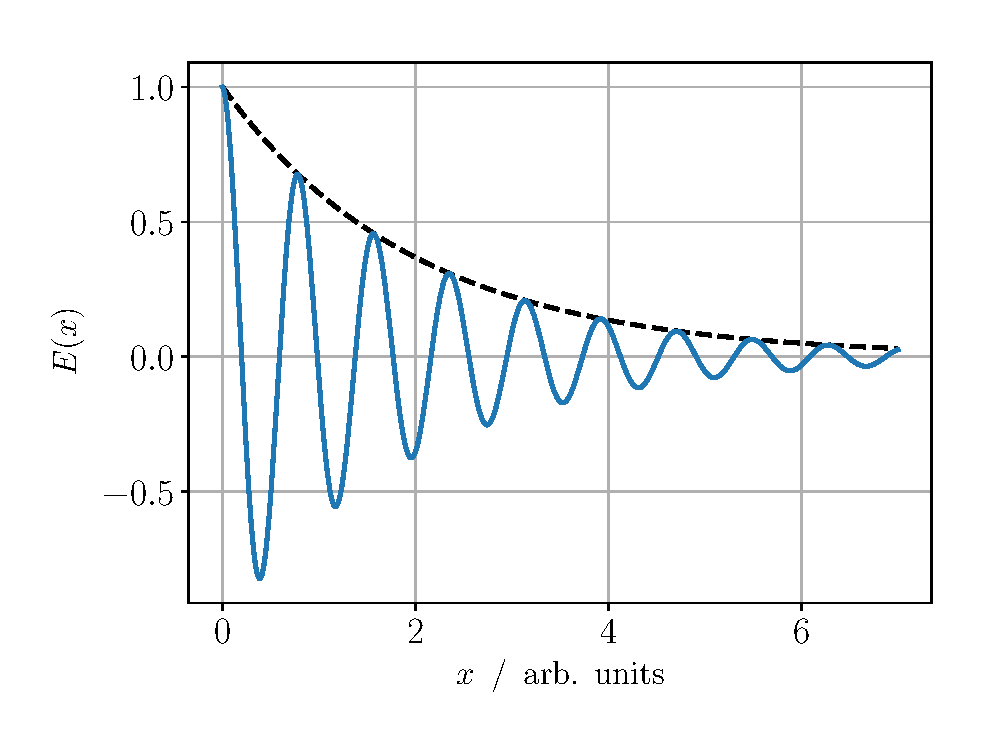
\includegraphics[width=.6\columnwidth]{Matematik/matfig/e-felt.eps}
    \caption{Det elektriske felt som funktion af afstanden fra materialets overflade til en fastsat tid. Her er $\kappa = 1/2$ og $k=n\omega/c=8$, hvor begge dele er i arbitrære enheder.}
    \label{mat:fig:e-felt}
\end{figure}
%%
%%
\begin{opgave}[3]{Eulers formel og komplekse tal på polær form}
Her skal vi arbejde med Eulers formel og prøve at få lidt intuition for, hvordan funktionen $e^{ix}$ opfører sig. I 5) skal I videre kigge på det, der kaldes for den polære form for komplekse tal.
\opg Tegn det komplekse tal $e^{ix}$ vha. Eulers formel \eqref{k-Eulers_formel} fra matematikafsnittet for $x=0, \, \pi/2, \, \pi, 3\pi/2$ (hvis ens lommeregner regner i grader for $\cos(x)$ og $\sin(x)$ skal man bruge $x=0, \, 90, \, 180, \, 270$ i stedet). Hvilken vej bevæger $e^{ix}$ sig rundt i den komplekse plan, når $x$ vokser?
\opg Ændres modulus af $e^{ix}$, hvis man ændre på $x$? Hint: Regn modulus af $e^{ix}$ vha. Eulers formel.
\opg Hvilken vej tror du, at $e^{-ix}$ bevæger sig rundt i den komplekse plan, når $x$ vokser?
\opg Ændres modulus af $e^{-ix}$, hvis man ændre $x$?
\opg Vis at ethvert komplekst tal $z = a+bi$ kan skrives på følgende form
\begin{align}
z = \abs{z}e^{i\theta} \, ,
\end{align} 
hvor $\theta = \tan^{-1}(b/a)$. Her er $\theta$ vinklen mellem den reelle akse og $z$ i det komplekse plan, og kaldes for $z$'s argument. I skal altså starte med $z=a+bi$ og omskrive, indtil i får noget på formen $|z|e^{i\theta}$. Denne måde at skrive et komplekst tal kaldes for den polære form.\\
Hint: Tegn $z$ i det komplekse plan og udtryk $a,b$ ved $\abs{z},\theta$ før I begynder at skrive om.
\end{opgave}
%%
%%
\begin{opgave}[3]{Komplekse tal og lys i materialer}
En vigtig ting i fysik er, at alle fysiske størrelser vi måler i laboratoriet, er reelle  tal. Komplekse tal er dog meget nyttige og dukker op over det hele. \\
Sender man lys ind i et materiale ændres lysets hastighed, hvilket er beskrevet ved lyset brydningsindeks, $n$, men noget af lyset vil også absorberes. Man kan vise at lysets elektriske feltstyrker en afstand $x$ inde i materialet til tiden $t$ er 
%
\begin{align} \label{mat:eq:e-felt-cos}
    E(x,t) = E_0e^{-\kappa x}\cos\left(\omega\left[\frac{n}{c}x-t\right]\right),
\end{align}
%
hvor $k$ er lysets bølgetal, $c$ er lyshastigheden og $\kappa$ kaldes attenuations- eller absorbtionskoefficienten, der beskriver hvor hurtigt feltstyrken aftager i mediet.
\opg Forklar hvordan de to kurver i \cref{mat:fig:e-felt} relaterer sig til \cref{mat:eq:e-felt-cos}.
\opg Hvordan ville figuren ændre sig, hvis man ændrede $\kappa$?
\opg Hvordan ville figuren ændre sig, hvis man ændrede $n$? \\[2mm]
I optik arbejder man ofte med et komplekst brydningsindeks, der kan defineres som $\tilde{n} = n + ic\kappa/\omega$, således at det elektriske felt kan skrives på den elegante form\footnote{Denne form er god, da eksponentialfunktionen i modsætning til cosinus har pæne regneregler, hvorfor den er markant lettere at arbejde med.}
%
\begin{align} \label{mat:eq:e-felt-exp}
    E(x,t) = \text{Re}\left\{E_0\exp\left(i\omega\left[\frac{\tilde{n}}{c}x - t\right]\right)\right\} = \text{Re}\left\{E_0e^{i\left(\tilde{k}x - \omega t\right)}\right\}.
\end{align}
\opg Vis at de elektriske felte i \cref{mat:eq:e-felt-cos,mat:eq:e-felt-exp} er lig hinanden.
\opg Hvilke tal i \cref{mat:eq:e-felt-exp} kan måles i et eksperiment? Er de reelle eller komplekse?
\end{opgave}